% =============================================================================
%  s03_seccion_modelo_analitico.tex — Sección 3: El Modelo Analítico
% =============================================================================

\section{El Modelo Analítico}

% ── Frame 3.1: El Origen: Un Problema de Puentes ─────────────────────────────
\begin{frame}{El Origen: Un Problema de Puentes}
  \begin{columns}[T]
    \begin{column}{0.55\textwidth}
      \begin{block}{\scriptsize Königsberg, 1736 — Leonhard Euler}
        \centering
        \includegraphics[width=\textwidth, height=4.0cm, keepaspectratio]%
          {../../../Tesis_Latex/Figures/Cap3/MapaKonisnberg.png}
      \end{block}
      \fuentefigura{\citep{garcia2005, braicovich2009}}
    \end{column}
    \begin{column}{0.42\textwidth}
      {\color{ColorAcento}\rule{0.9\textwidth}{1pt}}\\[0.15cm]
      {\tiny
        \textbf{El problema:} ciudad dividida en 4 zonas por el Pregel;
        7 puentes. ¿Puede alguien cruzarlos sin repetir ninguno?\\[0.1cm]
        \textbf{La abstracción de Euler:}\\
        zonas \(\rightarrow\) \textbf{nodos} \quad
        puentes \(\rightarrow\) \textbf{aristas}\\
        La geografía desaparece; la relación permanece.\\[0.1cm]
        \textbf{El resultado:} nació la Teoría de Grafos —
        aplicada a la \zmvm\ 300 años después.
      }\\[0.15cm]
      {\color{ColorAcento}\rule{0.65\textwidth}{0.8pt}}\\[0.15cm]
      {\scriptsize\bfseries\color{ColorPrincipal}
        La pregunta de Euler en 1736\\
        es la misma pregunta\\
        de esta tesis en 2026.}
    \end{column}
  \end{columns}
\end{frame}

% ── Frame 3.2: De la Ciudad al Grafo ─────────────────────────────────────────
\begin{frame}{De la Ciudad al Grafo}
  \begin{columns}[c]
    % ── Panel izquierdo: red física esquemática ───────────────────────────────
    \begin{column}{0.40\textwidth}
      \centering
      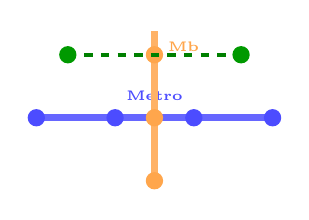
\begin{tikzpicture}[
        dot/.style  = {circle, minimum size=0.22cm, inner sep=0pt},
        ruta/.style = {line width=2.5pt},
      ]
        % Metro (azul, horizontal)
        \draw[ruta, blue!60] (0cm, 0.8cm) -- (3.0cm, 0.8cm);
        \foreach \x in {0, 1.0, 2.0, 3.0} {
          \node[dot, fill=blue!70] at (\x cm, 0.8cm) {};
        }
        \node[font=\tiny\bfseries, blue!70, above] at (1.5cm, 0.9cm) {Metro};
        % Metrobús (naranja, vertical)
        \draw[ruta, orange!60] (1.5cm, -0.1cm) -- (1.5cm, 1.9cm);
        \foreach \y in {0, 0.8, 1.6} {
          \node[dot, fill=orange!70] at (1.5cm, \y cm) {};
        }
        \node[font=\tiny\bfseries, orange!70, right] at (1.55cm, 1.7cm) {Mb};
        % RTP (verde, punteado)
        \draw[ruta, green!50!black, dashed, line width=1.5pt]
          (0.4cm, 1.6cm) -- (2.6cm, 1.6cm);
        \node[dot, fill=green!60!black] at (0.4cm, 1.6cm) {};
        \node[dot, fill=green!60!black] at (2.6cm, 1.6cm) {};
      \end{tikzpicture}\\[0.15cm]
      {\scriptsize\color{gray!60} Red física: trazados y geografía}
    \end{column}
    % ── Flecha central ────────────────────────────────────────────────────────
    \begin{column}{0.16\textwidth}
      \centering
      {\LARGE\color{ColorAcento}\(\Rightarrow\)}\\[0.1cm]
      {\tiny\bfseries\color{ColorAcento} abstracción}
    \end{column}
    % ── Panel derecho: grafo matemático ──────────────────────────────────────
    \begin{column}{0.40\textwidth}
      \centering
      \begin{tikzpicture}[
        nodo/.style   = {circle, draw=ColorPrincipal, fill=ColorPrincipal!20,
                         minimum size=0.55cm, font=\scriptsize\bfseries, inner sep=1pt},
        arista/.style = {draw=ColorPrincipal!70, line width=1.2pt},
        peso/.style   = {font=\tiny, fill=white, inner sep=1pt, color=ColorPrincipal},
      ]
        \node[nodo] (A) at (0cm, 0.8cm) {A};
        \node[nodo] (B) at (1.5cm, 1.6cm) {B};
        \node[nodo] (C) at (3.0cm, 0.8cm) {C};
        \node[nodo] (D) at (1.5cm, 0cm) {D};
        \draw[arista] (A) -- node[peso, above left]  {\(5'\)} (B);
        \draw[arista] (B) -- node[peso, above right] {\(8'\)} (C);
        \draw[arista] (A) -- node[peso, below left]  {\(3'\)} (D);
        \draw[arista] (D) -- node[peso, below right] {\(6'\)} (C);
        \draw[arista] (B) -- node[peso, right]       {\(4'\)} (D);
      \end{tikzpicture}\\[0.15cm]
      {\scriptsize\color{gray!60} Grafo: nodos, aristas, pesos de tiempo}
    \end{column}
  \end{columns}
  \vspace{0.2cm}
  {\small\color{ColorPrincipal}
    El grafo no mide kilómetros — mide
    \textbf{tiempo, transferencias y vulnerabilidad}.
    Sobre esa estructura operan los algoritmos del modelo.}
\end{frame}

% ── Frame 3.3: Los 3 Indicadores ─────────────────────────────────────────────
\begin{frame}{Los 3 Indicadores: ¿Qué Mide el Modelo?}
  \begin{columns}[T]
    % ── DI ────────────────────────────────────────────────────────────────────
    \begin{column}{0.31\textwidth}
      \begin{block}{\scriptsize DI — Índice de Rodeo}
        \centering
        \includegraphics[width=\textwidth, height=2.2cm, keepaspectratio]%
          {../../../Tesis_Latex/Figures/Cap3/DistanciaEuclidiana.png}\\[0.1cm]
        \tiny ¿Qué tan tortuoso es el viaje real vs.\ la línea recta?
        DI alto = la red obliga a dar rodeos innecesarios.
      \end{block}
      \fuentefigura{Base: \citet{fortin2016innovative}}
    \end{column}
    % ── B(v) ──────────────────────────────────────────────────────────────────
    \begin{column}{0.31\textwidth}
      \begin{block}{\scriptsize B(v) — Intermediación}
        \centering
        \includegraphics[width=\textwidth, height=2.2cm, keepaspectratio]%
          {../../../Tesis_Latex/Figures/Cap3/CentralidadItnermediacion.png}\\[0.1cm]
        \tiny ¿Qué tan indispensable es una estación?
        B(v) alto = si falla, muchos viajes
        se interrumpen.
      \end{block}
      \fuentefigura{Base: \citet{lee2008}}
    \end{column}
    % ── ΔE ────────────────────────────────────────────────────────────────────
    \begin{column}{0.31\textwidth}
      \begin{block}{\scriptsize $\Delta E$ — Robustez}
        \centering
        \includegraphics[width=\textwidth, height=2.2cm, keepaspectratio]%
          {../../../Tesis_Latex/Figures/Cap3/RobustezGeometrica.png}\\[0.1cm]
        \tiny ¿Cuánto cae la eficiencia si se elimina un nodo?
        Mide el peor escenario posible.
      \end{block}
      \fuentefigura{Base: \citet{loterovélez2014}}
    \end{column}
  \end{columns}
  \vspace{0.15cm}
  {\small\itshape\color{ColorPrincipal}
    Juntos responden: ¿dónde está el problema, quién lo causa
    y qué tan grave sería perderlo?}
\end{frame}

% ── Frame 3.4: El Pipeline ────────────────────────────────────────────────────
\begin{frame}{El Pipeline: De los Datos a los Resultados}
  \vspace{0.35cm}
  \begin{center}
  \begin{tikzpicture}[
    paso/.style   = {rectangle, rounded corners=4pt,
                     draw=gray!50, line width=0.8pt,
                     fill=gray!10, text=gray!60,
                     text width=1.65cm, align=center,
                     minimum height=0.82cm, font=\scriptsize\bfseries},
    propio/.style = {rectangle, rounded corners=4pt,
                     draw=ColorPrincipal, line width=1pt,
                     fill=ColorPrincipal, text=white,
                     text width=1.65cm, align=center,
                     minimum height=0.82cm, font=\scriptsize\bfseries},
    desc/.style   = {text width=1.65cm, align=center,
                     font=\tiny, text=gray!65},
    flecha/.style = {-Stealth, thick, color=ColorAcento},
  ]
    \node[paso]   (g1) {\textbf{01}\\[1pt]GTFS};
    \node[propio, right=0.25cm of g1] (g2) {\textbf{02}\\[1pt]Apimetro};
    \node[paso,   right=0.25cm of g2] (g3) {\textbf{03}\\[1pt]Grafo};
    \node[propio, right=0.25cm of g3] (g4) {\textbf{04}\\[1pt]VFTModel};
    \node[paso,   right=0.25cm of g4] (g5) {\textbf{05}\\[1pt]Resultados};

    \draw[flecha] (g1.east) -- (g2.west);
    \draw[flecha] (g2.east) -- (g3.west);
    \draw[flecha] (g3.east) -- (g4.west);
    \draw[flecha] (g4.east) -- (g5.west);

    \node[desc, below=0.35cm of g1]
      {Datos abiertos: Metro, Metrobús, RTP, Tren Ligero};
    \node[desc, below=0.35cm of g2]
      {Limpia GTFS y expone la red como API REST};
    \node[desc, below=0.35cm of g3]
      {Nodos y aristas con pesos temporales};
    \node[desc, below=0.35cm of g4]
      {Calcula DI, B(v) y $\Delta E$; simula el anillo};
    \node[desc, below=0.35cm of g5]
      {Indicadores cuantitativos + mapas QGIS};
  \end{tikzpicture}
  \end{center}
  \vspace{0.15cm}
  {\scriptsize\itshape\color{gray!55}
    Los nodos en \textcolor{ColorPrincipal}{\textbf{verde}} son herramientas de autoría propia. · Elaboración propia.}
\end{frame}

% ── Frame 3.5: Apimetro y VFTModel ───────────────────────────────────────────
\begin{frame}{Apimetro y VFTModel — Herramientas de Investigación}
  \begin{columns}[T]
    % ── Imagen literaria ──────────────────────────────────────────────────────
    \begin{column}{0.42\textwidth}
      \begin{block}{\scriptsize La Saga de la Catacumba}
        \centering
        
\includegraphics[width=\textwidth, height=4.0cm, keepaspectratio]{LH15.png}
      \end{block}
      {\scriptsize\itshape\color{gray!65}
        \textit{La Historia de Quince} — uncronía urbana donde
        el tiempo de viaje es un recurso de equidad social.}
    \end{column}
    % ── Logos y texto ─────────────────────────────────────────────────────────
    \begin{column}{0.54\textwidth}
      \centering
      
\includegraphics[width=0.62\textwidth, height=1.2cm, keepaspectratio]{ApimetroLogo.png}\\[0.05cm]
      {\scriptsize\bfseries\color{ColorPrincipal} Apimetro}\\[0.03cm]
      {\tiny Consume GTFS y expone la red de Metro como API REST
        geoespacial navegable.}\\[0.12cm]
      {\color{ColorAcento}\rule{0.75\textwidth}{0.5pt}}\\[0.12cm]
      
\includegraphics[width=0.62\textwidth, height=1.2cm, keepaspectratio]{VFTLogo1.png}\\[0.05cm]
      {\scriptsize\bfseries\color{ColorPrincipal} VFTModel — \textit{Vanishing Fig-Tree}}\\[0.03cm]
      {\tiny Calcula DI, B(v) y $\Delta E$; simula la inserción
        del corredor anillar.}\\[0.12cm]
      {\color{ColorAcento}\rule{0.9\textwidth}{0.5pt}}\\[0.1cm]
    \end{column}
  \end{columns}
\end{frame}
